\documentclass[answers,addpoints,11pt]{exam}
\usepackage[utf8]{inputenc}
\usepackage[english]{babel}
\usepackage{listings}
\usepackage{amsmath}
\usepackage{algpseudocode}
\usepackage{graphicx}
\usepackage{amssymb}
\usepackage{amsthm}
\usepackage{hyperref}
\usepackage{logicproof}
\usepackage{multicol}
\usepackage{environ}
\usepackage{xcolor}
\usepackage{tikz}
\usetikzlibrary{arrows}
\usepackage{MnSymbol}

\tikzset{
  treenode/.style = {align=center, inner sep=0pt, text centered,
    font=\sffamily},
  nd_w/.style = {treenode, circle, black, draw=black, text width=1em, very thick},% node
  nd_filled/.style = {treenode, circle, black, draw=black, fill=gray, text width=1em, very thick},% node
  nd_b/.style = {treenode, circle, white, font=\sffamily\bfseries, draw=black,fill=black, text width=1em},% arbre rouge noir, noeud noir
  nd_r/.style = {treenode, circle, red, draw=red, text width=1em, very thick},% arbre rouge noir, noeud rouge
  nd_nil/.style = {treenode, rectangle, draw=black, fill=black, minimum width=0.5em, minimum height=0.5em}% null
}

\newcommand{\limit}[1]{ \lim_{n \rightarrow \infty} \left( #1 \right) }
\bracketedpoints
\qformat{Question \thequestion{} : \totalpoints{} \points \hfill}

%These setting will make the code areas look Pretty
\lstset{
	escapechar=~,
	numbers=left, 
	%numberstyle=\tiny, 
	stepnumber=1, 
	firstnumber=1,
	%numbersep=5pt,
	language=C,
	stringstyle=\itfamily,
	%basicstyle=\footnotesize, 
	showstringspaces=false,
	frame=single
}

\title{CS260 - Data Structures \\ Written Assignment 2}
\author{Fitsum Alebachew fa496} 
\date{}

\begin{document}
\maketitle

\begin{questions}
%%%%%%%%%%%%%%%%%%%%%%%%%%
%%%% Question 1 %%%%%%%%%%
%%%%%%%%%%%%%%%%%%%%%%%%%%
\question
It's just another day in your internship at Google. You feel like life starting to get mundane as you are thirsty of a new challenge. What you were looking for arrives sooner than you expect, from an unexpected direction though: Binary Search Trees. Answer the following questions on BSTs:

\begin{parts}
 \part[5] Bob is another intern working in the same group as you. He was assigned the job of designing and implementing a binary search tree (BST), which he did in a very short amount of time, becoming the favourite intern of the group leader. However, you have a gut feeling that, BST's that Bob's code generates do not always satisfy the BST property. Not out of jealousy, of course, but for your good will towards your employer, you mentioned your concerns to the group leader. She assigned you the job of developing an algorithm, which will test whether a given BST is valid or not. \\
 
 Suggest an algorithm in plain English that tests whether a given binary tree is a valid binary search tree. Also do the runtime analysis of your algorithm.
 \begin{solution}
 A recursive algorithm can be made that you pass the root of the tree to. It first checks if left child is less and right child is more than the parent, returning with error status otherwise. Then if the left and right child exist, it will recursively call the same function on them one by one. A check is made for every node by the end of this algorithm, so it has a runtime of $O(n)$.
 \end{solution}
 
 \part[5] Realizing your algorithm design skills, your group leader decided to test your boundaries. Although she is now convinced that you know something about BSTs (at least more than Bob), she wants to make sure that you understand the matter and do not "memorize" these data structures and algorithms. To further test the depth of your understanding in BST, she is now asking you to develop an algorithm that would determine whether two sets of keys that represent two BSTs are the same BSTs, without building the BSTs.\\
 
 Provide an example for two sets of keys $A={a_1,a_2,...,a_k}$ and $A'={a_1,a_5,a_7...,a_k}$, that are different in order but having the same set of elements, yet generate the same BST if inserted in order. You can assume that the elements will be integers.
 
 \begin{solution}\\
 A = 2, 1, 3, 4, 6\\
 A' = 2, 3, 4, 6, 1
 \end{solution}
 
 \part[5] As a follow up to part b above, suggest an algorithm in plain English and/or pseudocode that determines whether the two sets represent the same BST. Also do the runtime analysis of your algorithm.
 
 \begin{solution}
 The only way the end result is the same with a different order of elements is if the order of left and right children as seen from any parent is switched in the initial list. In other words, for every element the next smaller and the next larger elements should be consistent between the two arrays. The algorithm recursively iterates through each element in the arrays and finds the next smaller/larger element which takes $O(n)$ time. This makes this algorithm $O(n^2)$
 \end{solution}
\end{parts}

%%%%%%%%%%%%%%%%%%%%%%%%%%
%%%% Question 2 %%%%%%%%%%
%%%%%%%%%%%%%%%%%%%%%%%%%%
\question
Your project leader has been quite impressed by your performance on binary search trees, and started entertaining the idea of keeping you full time after you graduate. However, she needs to make a case to her manager about how magnificent a problem solver you are. Thus, she decided to put a few more challenges for you. This time she wants to test how well versed you are with heaps. You are given an unsorted array of size $n$. Below are the set of questions that you need to solve to prove your worth by using this unsorted array.
\begin{parts}
 \part[2] The naive way of generating a heap with that array is by using a separate list of the same size and generating the heap by inserting elements one by one. Give a $O(n\log n)$ time algorithm to generate the heap.
 \begin{solution}
 We start with a size variable initialized to zero. Then we insert an element to the new array at location 'size'. We then upheap the element to its correct place in the heap, after which we increase the size variable. We iterate through the initial array and do the same for every element. We will have the heap generated at the end of this in $O(n\log_2n)$ time.
 \end{solution}
 
 \part[8] That was easy. How about generating the heap in place? Give pseudocode or explain in plain English of a function, that generates a heap without using a second list. You can only use upheap/downheap functions that we used in class, while other functions (such as insert/deleteMin) are not allowed. What is the runtime of your algorithm?
 \begin{solution}
 We can use the downheap function to do this. We iterate through the list starting from the end and downheap each element up to the start. This ensures that each element is in the right spot. (runtime explained in part c)
 \end{solution}
 
\part[5] Although we stated that generating the heap would take $O(n\log n)$ above, it was actually a loose bound which assumes that each insertion will take $O(\log n)$ time, for each of the $n$ insertions. However, as you might have noticed when going though your iterations in the previous part of the problem, fixing the heap property for some nodes (or with the similar idea, inserting elements to a heap in early stages) do not always take $O(\log n)$ where, $n$ is the size of the final heap. In fact, earlier stages takes less time, revealing that our initial $O(n\log n)$ time might have been a loose bound. Make a careful analysis of the make heap algorithm and show that it has $O(n)$ time.
\begin{solution}
 The last row of the heap can not be downheaped. As we go up in the heap, The row above it will have $n/4$ elements that all take one swap maximum, and the $n/8$ elements above those take 2 swaps maximum. The total swaps will be $n/4 + 2n/8 + 3n/16 + ... + \log n$. The infinite series $1/4 + 2/8 + 3/16 + ...$ is the converging power series $n/2^n^+^1$. Since the coefficients of n in total swap are part of this series, it too must be a finite number. A finite multiple of n will make it $O(n)$.
 \end{solution}

\end{parts}


%%%%%%%%%%%%%%%%%%%%%%%%%%
%%%% Question 3 %%%%%%%%%%
%%%%%%%%%%%%%%%%%%%%%%%%%%
\question
Below is a set of questions that would test the boundaries of your red-black trees understanding.\\

A valid Red-Black tree should satisfy the following 5 requirements:
\begin{enumerate}
    \item Every node is either red or black.
    \item The root is black.
    \item Every leaf is NULL and black.
    \item If a node is red, then both its children are black. 
    \item All paths from a node x to any leaf have same number of black nodes in between (i.e., their Black-Height(x) is the same)
\end{enumerate}
After insertion of a new key $x$ to the tree, properties 3 and 5 can get violated, which requires re-balancing of the tree. Following are the possible cases of violation for the red-black properties:\\
\begin{enumerate}
    \item $x$’s parent is the left child of $x$’s grandparent while $x$’s uncle is Red.
    \item $x$’s parent is the left child of $x$’s grandparent, $x$’s uncle is Black, and $x$ is right child of its parent.
    \item $x$’s parent is the left child of $x$’s grandparent, $x$’s uncle is Black, and $x$ is the left child of its parent.
    \item $x$’s parent is the right child of $x$’s grandparent while $x$’s uncle is Red.
    \item $x$’s parent is the right child of $x$’s grandparent, $x$’s uncle is Black, and $x$ is right child of its parent.
    \item $x$’s parent is the right child of $x$’s grandparent, $x$’s uncle is Black, and $x$ is the left child of its parent.
\end{enumerate}
These violations can be overcome by rotating the tree around certain nodes and making updates in their colors, as described in the slides. First three of these cases along with how to handle them were described in the slides, from which you can deduce how to handle the rest, as the latter three are the mirroring cases of the former three.

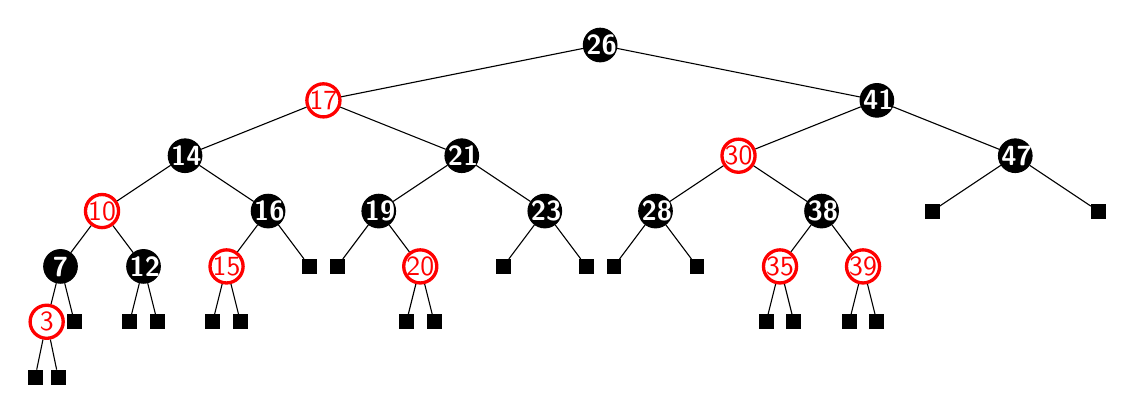
\begin{tikzpicture}[-,>=stealth',level 1/.style={sibling distance=20em},level 2/.style={sibling distance=10em},level 3/.style={sibling distance=6em},level 4/.style={sibling distance=3em},level/.style={sibling distance = 5em/#1, level distance = 2em}] 
\node [nd_b] {26}
    child{ node [nd_r] {17} 
        child{ node [nd_b] {14} 
        	child{ node [nd_r] {10}
        	    child{ node [nd_b] {7}
        	        child{ node [nd_r] {3}
        	            child{ node [nd_nil] {}}
        	            child{ node [nd_nil] {}}
        	        }
        	        child{ node [nd_nil] {}}
        	    }
        	    child{ node [nd_b] {12}
        	        child{ node [nd_nil] {}}
        	        child{ node [nd_nil] {}}
        	    }
        	} 
			child{ node [nd_b] {16}
			    child{ node [nd_r] {15}
        	        child{ node [nd_nil] {}}
        	        child{ node [nd_nil] {}}
        	   }
        	   child{ node [nd_nil] {}}
			}
        }
        child{ node [nd_b] {21}
			child{ node [nd_b] {19}
			    child{ node [nd_nil] {}}
			    child{ node [nd_r] {20}
			        child{ node [nd_nil] {}}
			        child{ node [nd_nil] {}}
			    }
			}
			child{ node [nd_b] {23}
		        child{ node [nd_nil] {}}
		        child{ node [nd_nil] {}}
		    }
        }                            
    }
    child{ node [nd_b] {41}
        child{ node [nd_r] {30} 
			child{ node [nd_b] {28}
			    child{ node [nd_nil] {}}
		        child{ node [nd_nil] {}}
			}
			child{ node [nd_b] {38}
			    child{ node [nd_r] {35}
			        child{ node [nd_nil] {}}
		            child{ node [nd_nil] {}}
			    }
		        child{ node [nd_r] {39}
		            child{ node [nd_nil] {}}
		            child{ node [nd_nil] {}}
		        }
			}
        }
        child{ node [nd_b] {47}
			child{ node [nd_nil] {}}
			child{ node [nd_nil] {}}
        }
	}
; 
\end{tikzpicture}

\begin{parts}
\part[5] Considering the Red-Black tree given above, insert the key 36 to this tree. Which cases are you going to encounter? What rotations would you need to overcome these cases? What would the final tree look like? (Note: It suffices to show the final state in picture, but explain verbally what rotations you will do to achieve to that state due to which violations)
\begin{solution}
 36 will be the right child of 35. This makes its parent the left child of its grandparent, and its uncle which is 39 is red (case 1). We toggle the colors of 35, 38 and 39. Then we get case 2 with 38. We then do a rotation bringing 38 up and 41 as its left child, while 38's right children become 41's left children. Final tree below.\\
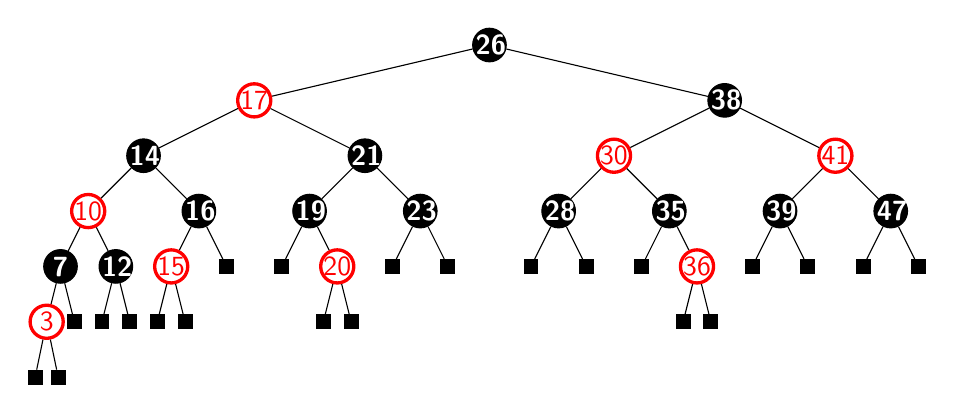
\begin{tikzpicture}[-,>=stealth',level 1/.style={sibling distance=17em},level 2/.style={sibling distance=8em},level 3/.style={sibling distance=4em},level 4/.style={sibling distance=2em},level/.style={sibling distance = 5em/#1, level distance = 2em}] 
\node [nd_b] {26}
    child{ node [nd_r] {17} 
        child{ node [nd_b] {14} 
        	child{ node [nd_r] {10}
        	    child{ node [nd_b] {7}
        	        child{ node [nd_r] {3}
        	            child{ node [nd_nil] {}}
        	            child{ node [nd_nil] {}}
        	        }
        	        child{ node [nd_nil] {}}
        	    }
        	    child{ node [nd_b] {12}
        	        child{ node [nd_nil] {}}
        	        child{ node [nd_nil] {}}
        	    }
        	} 
			child{ node [nd_b] {16}
			    child{ node [nd_r] {15}
        	        child{ node [nd_nil] {}}
        	        child{ node [nd_nil] {}}
        	   }
        	   child{ node [nd_nil] {}}
			}
        }
        child{ node [nd_b] {21}
			child{ node [nd_b] {19}
			    child{ node [nd_nil] {}}
			    child{ node [nd_r] {20}
			        child{ node [nd_nil] {}}
			        child{ node [nd_nil] {}}
			    }
			}
			child{ node [nd_b] {23}
		        child{ node [nd_nil] {}}
		        child{ node [nd_nil] {}}
		    }
        }                            
    }
    child{ node [nd_b] {38} 
		child{ node [nd_r] {30}
		    child{ node [nd_b] {28}
		        child{ node [nd_nil] {}}
	            child{ node [nd_nil] {}}
		    }
	        child{ node [nd_b] {35}
		        child{ node [nd_nil] {}}
	            child{ node [nd_r] {36}
	                child{ node [nd_nil] {}}
	                child{ node [nd_nil] {}}
	            }
		    }
		}
		child{ node [nd_r] {41}
            child{ node [nd_b] {39}
	            child{ node [nd_nil] {}}
	            child{ node [nd_nil] {}}
	        }
            child{ node [nd_b] {47}
    			child{ node [nd_nil] {}}
    			child{ node [nd_nil] {}}
            }
    	}
    }
; 
\end{tikzpicture}
 \end{solution}

\part[5] What is the asymptotic cost of inserting a new key to a red-black tree? Explain your answer.
\begin{solution}
 Solving one case takes $O(1)$ time since a finite amount of manipulations are done, not depending on the size of the tree. Each solve has the chance of creating another case above it, this might ripple all the way to the top. This makes it $O(h)$ in the worst case where h is the height of the tree: $O(2\log (n+1))$. 
 \end{solution}

\part[5] Where would you use red-black trees? Why?
\begin{solution}
 Red black trees are one way of achieving a balanced tree because its height is $2\log (n+1)$ max. This helps make the run time of tree operations lower because the height of a tree can go upto n in the worst case.
 \end{solution}
 
\end{parts}

%%%%%%%%%%%%%%%%%%%%%%%%%%
%%%% Question 4 %%%%%%%%%%
%%%%%%%%%%%%%%%%%%%%%%%%%%
\question
Answer the following questions about graphs.

\begin{parts}
\part[3] What is the maximum number of edges that can exist in an undirected graph? Why? Explain.
\begin{solution}
 If every vertex is interconnected, the graph will have $1+2+...+(n-1)$ edges, which is $n(n-1)/2$ edges.
 \end{solution}
\part[3] What is a cycle in a directed graph?
\begin{solution}
 A cycle is a path that ends at its starting vertex.
 \end{solution}
\part[3] Given a graph $G(V,E)$, its inverse consists of a graph $G'$ where the edges of the original graph is inverted. That is, for all $(u,v) \in G.E$, $\exists (v,u) \in G'.E$. Describe a nonempty directed graph $G$ such that $G=G'$.
\begin{solution}
 A directed graph with a symmetric adjacency matrix will have the same inverse. It is a graph where for every edge from a to b, there is an edge from b to a.
 \end{solution}
\part[3] Topological sorting in a directed graph is a linear ordering of its vertices. Does existence of a cycle in a graph violate a topological sorting? Why/why not?
\begin{solution}
 Yes, any linear ordering of a graph with a cycle will have a back edge, meaning the order is not sorted topologically. So it will not be possible to find an order that works.
 \end{solution}
\part[3] Depth First Search can be used as a subroutine to solve other problems, topological sorting being an example of this. Explain the intuition behind using DSF in the calculation of topological sort. (Note: I'm not asking you about how DFS is used in topological sorting. Rather, I'm asking what is needed to topologically sort graphs and how DFS becomes useful to achieve this)
\begin{solution}
 In DFS, a parent (predecessor) does not get finishing time (black color) before its children(things that must come after in the final order). Using DFS with topological sorting ensures that the children come first in the final ordering since items are added in the head of the list as they are finished (colored black).
 \end{solution}
\end{parts}

%%%%%%%%%%%%%%%%%%%%%%%%%%
%%%% Question 5 %%%%%%%%%%
%%%%%%%%%%%%%%%%%%%%%%%%%%
\question
A {\it strongly connected component} (SCC) of a directed graph $G(V,E)$ is a maximal set of vertices $C \subseteq V$ such that for every pair of vertices $u$ and $v$ in $C$, we have both $u \leadsto v$ and  $v \leadsto u$; that is, vertices $u$ and $v$ are reachable from each other.\\
In the example graph given below, the sets of nodes ${a,b,e}$, ${c,d}$,  ${f,g}$,  and ${h}$ each form a strongly connected component. Thus, the graph consists of 4 strongly connected components.\\
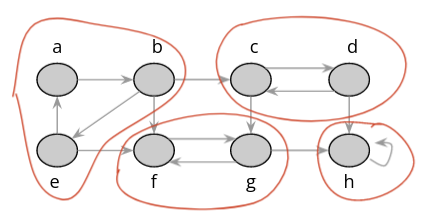
\includegraphics[width=8cm]{scc.png}

\begin{parts}
\part[7] Breadth First Search (BFS) can be used in determining whether each node in a given directed graph is reachable by every other node.  Give the pseudocode of an algorithm using BFS that determines whether a given directed graph is a single SCC. Also provide the explanation of your algorithm in plain English along with a runtime analysis.
\begin{solution}
 \begin{lstlisting}[escapeinside={(*}{*)}]
  color_all_nodes_white
  for V in G.V
    BFS(V)
    if (v.color = = white) for v in G.V
        return 0
    color_all_nodes_white
  return 1
 \end{lstlisting}\\
 The algorithm does a BFS traversal for every node in the graph. For each iteration, if there is a node that has not been visited, it means that the graph is not a single SCC.\\
 It has a runtime of $O(V(V + E))$ since BFS is ran for each vertex.
 \end{solution}
\part[8] Depth First Search (DFS) can be used to calculate strongly connected components in a graph. Give the pseudocode of an algorithm using DFS that calculates SCCs in a given directed graph. Also provide the explanation of your algorithm in plain English along with a runtime analysis.
\begin{solution}
 \begin{lstlisting}[escapeinside={(*}{*)}]
 stack = {}
 DFS(G){
    add2stack(visited_node);
 }
 G.E = transpose(G.E)
 while(stack_not_empty){
    node=pop(stack)
    DFSvisit(node){
        print(visited_node)
    }
 }
\end{lstlisting}\\
The algorithm does a DFS traversal on the graph and adds the visited nodes into a stack. Then, it reverses the edges in the graph and does DFS on the new graph again using the popped elements of the stack as the starting point.\\
It takes $O(V + E)$ time since both DFS and reversing a graph take $O(V+E)$ time.
 \end{solution}
\end{parts}

%%%%%%%%%%%%%%%%%%%%%%%%%%
%%%% Question 6 %%%%%%%%%%
%%%%%%%%%%%%%%%%%%%%%%%%%%
\question
You are given a weighted undirected graph $G=(V,E)$, where $E$ and $V$ denote set of edges and vertices, and a minimum spanning tree $T$ of that graph $G$. Answer the following questions about $G$ and $T$ on minimum spanning trees.
\begin{parts}
 \part[5] Suppose we decrease the weight of one of the edges in $G$ that is not among the edges in $T$. Suggest an algorithm in plain English that determines whether $T$ is still a minimum spanning tree, and if it is not, calculates a minimum spanning tree of $G$. Explain the running time of your algorithm. (Note: Your algorithm should be faster than Prim's and Kruskal's) 
\begin{solution}
 Let us add the edited edge into the MST. The MST(no longer an MST) has exactly one cycle. We get the new MST when we remove the node with the highest weight from this cycle (we can use DFS to find the cycle). If the highest weight edge in the cycle is the edited edge, then the MST has not changed. If the highest weight edge is any other element, then we have a new MST. This algorithm has $O(n)$ running time, since finding the cycle and finding the highest element both take $O(n)$ time.
 \end{solution}
 
 \part[5] Consider the following algorithm running on $G=(V,E)$. Would it calculate a valid MST of $G$? If yes, explain your reasoning in plain English, if no, provide a counter example graph that the algorithm will fail producing an MST. Also, what is the running time of the algorithm in the previous question. Show your analysis.
 
 \begin{lstlisting}[escapeinside={(*}{*)}]
MSTcandidate(G)
 E = sort G.E in decreasing order of edge weights
 T = E
 for i from 1 to |E| do
    if T - {E[i]} is a connected graph
        T = T - {E[i]}
    end if
 end for
 return T
\end{lstlisting}

\begin{solution}
 Yes\\
 By the end of this algorithm, every node is checked to see if they are necessary for a connected graph and removes if otherwise. This means we will surely have a spanning tree. Since the iteration goes from highest weight edges to least, every removed edge will be the highest possible total weight reduction. Thus by the end, we will have both a spanning tree and the least total weight, i.e. an MST.
 \end{solution}

 \end{parts}

\newpage 

%%%%%%%%%%%%%%%%%%%%%%%%%%
%%%% Question 7 %%%%%%%%%%
%%%%%%%%%%%%%%%%%%%%%%%%%%
\question
In economics, arbitrage is the practice of taking advantage of a difference in prices in two or more markets; striking a combination of matching deals to capitalize on the difference, the profit being the difference between the market prices at which the unit is traded.\\

Arbitrage can become a source of gain when applied to currency exchanges. Consider the following currency exchange ratios as an example: 1 U.S. dollar buys 0.7292 euros, 
1 euro buys 105.374 Japanese yen, 1 Japanese yen buys 0.3931 Russian rubles, 1 Russian ruble buys 0.0341 U.S. dollars.\\

Then you could take 1 U.S. dollar and buy 0.7292 euros with it, with which you can buy 76.8387 yen (because 0.7292 * 105.374 = 76.8387). Then take the 76.8387 yen and buy 30.2053 rubles (because 76.8387 * 0.3931 = 30.2053), and finally take the 30.2053 rubles and buy 1.03 dollars (because 30.2053 * 0.0341 = 1.0300). \\

Assume that you are given the pairwise trading ratios among $n$ currencies and answer the following questions about arbitrage accordingly.

\begin{parts}
\part[5] Describe the problem as a graph problem. What are your nodes? What are the edges? Is this a weighted graph? Is the graph directed? What is the goal over this graph?
\begin{solution}
 The problem would involve a directed graph with the currencies as the nodes and the exchange rate being the weights of the edges, pointing from the node of the currency being exchanged to the node of the currency being bought. The goal is to find a path where the product of edge weights is greater than 1.
 \end{solution}
\part[5] Suggest an algorithm in plain English that evaluate whether an arbitrage exists among these $n$ currencies.
\begin{solution}
 The algorithm would use the same graph mentioned above but edit the edges to their log values. This means the sum of these edges will be the log of the product of the exchange rates. If the sum of edges exceeds 0, then the product exceeds 1. DFS can be used to find cycles within the graph, and when the back edge is encountered, the sum of the edges in the cycle will tell us if there is an arbitrage or not.
 \end{solution}
\part[5] Expand your algorithm so that it prints the chain of arbitrage and analyze the running time of your algorithm.
\begin{solution}
 When an arbitrage is found, we can start backtracking and saving the chain until we reach the initial node(currency). The arbitrage chain will be the reverse of this list, since we started from the end.
 \end{solution}

\end{parts}


\end{questions}
\end{document}